\chapter{复数}
谁说$\Delta < 0$就没有解,\gls{complex}十分生气地说。

\section*{学习目标}
\begin{todolist}
\item 理解复数的概念,以及相关定义。包括实部,虚部,模,\gls{arg},\gls{conj}等相关概念
\item 进行复数的加减乘除运算
\item 理解复数是可以充当某个多项式的非实数解,并且该复数的共轭复数也是多项式的解。
\item 利用\gls{arg diagram}表示复数,并且能够解释复数的模和幅角的几何意义
\item 理解复数的两种表示方法Cartesian Form和Polar Form。以及两者之间的联系
\item 从阿干特图的角度理解共轭复数,以及复数的加减乘除的几何含义
\item 掌握欧拉公式和棣莫弗公式
\item 以Polar Form的形式求算复数的乘除法,以及求算复数的平方根
\item 通过复数的方程或者不等式绘制复数的\gls{loci}
\end{todolist}
\clearpage

\section{复数的基本概念}
要引入复数的话,我们首先要学习虚数以及\gls{imag}单位的概念,因此就要回到最早的二次方程当中。
\[
	x^2=-1
\]
这样的一个方程,是没有\emph{实数解}的。因此任何实数,无论是正是负,其平方都是正数。所以这个方程就无解了。可是数学家作为一群坚信只要有问题就有答案的一群人(知乎,请结算广告费),强行把该方程的解记做$\mathbf{i}=\sqrt{-1}$。这个数不属于之前的实数范畴,是人为创造出来的数字。因此叫做Imaginary Number。一旦可以接受这个虚数单位的概念之后。负数就可以开根了。

\subsection*{复数作为根}
因此,对于$(x-3)^2=-4$这种没有实数解的二次方程,可以使用虚数进行求算。其结果为$x=3+\sqrt{4}\mathbf{i}$和$x=3-\sqrt{4}i$。而这样的数字就是这个章节的绝对主角——复数。

\begin{definition}
 $z=a+ib$ is called a complex number. $a$ is called the real part, and $b$ is called imaginary part.
\end{definition}
在这里要注意,只有$b$才是虚部,不包含$\mathbf{i}$,$\mathbf{i}$是虚数单位。

\subsection*{共轭复数}
如果两个复数\textbf{实部相同,虚部相反}。这两个复数就被称之为彼此的共轭复数。标记手段为$z=a+\mathbf{i}b, z^*=a-\mathbf{i}b$

\subsection*{复数的加减乘除运算}
既然复数也是一种数,就有基本的运算法则:

\subsubsection*{加法与减法}
两个复数相加相减,只需要把实部相加或者相减,作为结果的实部;把虚部相加减作为结果的虚部即可。
\begin{TaskBox}
 $z_1=3+2\mathbf{i}$, $z_2=5-4\mathbf{i}$,求算$z_1+z_2$ 和$z_2-z_1$
\end{TaskBox}

\subsubsection*{复数的乘法}
两个复数相乘,需要利用乘法的分配律打开括号进行合并化简。
\begin{ExampleBox}
 $z_1=3+2\mathbf{i}$, $z_2=5-4\mathbf{i}$,求算$z_1\cdot z_2$
\tcblower
 \begin{align*}
 	z_1\cdot z_2 &= (3+2\mathbf{i})\cdot (5-4\mathbf{i}) \\
 				 &= 3\times 5 +2\mathbf{i}\times 5-3\times 4\mathbf{i}-2\mathbf{i}\times 4\mathbf{i}\\
 				 &=15 +10\mathbf{i} -12\mathbf{i} -8i^2\\
 				 &=15+8 +(10-12)\mathbf{i}\\
 				 &=23-2\mathbf{i}
 \end{align*}
\end{ExampleBox}

所以,复数的乘法本质上就是将实部和虚部分别相乘再进行合并而已。

\begin{TaskBox}
 证明:共轭复数$z\cdot z^*$的最终结果是一个实数$a^2+b^2$
\end{TaskBox}

\subsubsection*{复数的除法}
既然两个复数相乘可以得到结果比如$(3+2\mathbf{i})\cdot (5-4\mathbf{i})=23-2\mathbf{i}$,那么理论上$(23+2\mathbf{i})\div(3+2\mathbf{i})$必然是可以求算的,且结果为$5-4\mathbf{i}$,因此也可以计作$\frac{23-2\mathbf{i}}{3+2\mathbf{i}}=5-4i$。How comes?
在这里采用的思想是利用之前的结论,就是因为分母不是一个实数,不太好直接相除,因此如果分子分母同时乘某一个数,分母可以成为实数的话,那不就好了。应用共轭复数的结论,就可以做复数的除法了,同时这个过程也被称之为分母实数化。
\begin{ExampleBox}
证明上述的除法
\tcblower
\begin{align*}
	\frac{23+2\mathbf{i}}{3+2\mathbf{i}} &= \frac{(23-2\mathbf{i})\cdot (3-2\mathbf{i})}{(3+2\mathbf{i})\cdot(3-2\mathbf{i})}\\
					   &=\frac{69-6\mathbf{i}-46\mathbf{i}+4\mathbf{i}^2}{3^2+2^2}\\
					   &=\frac{65-52\mathbf{i}}{13}\\
					   &=5-4\mathbf{i}
\end{align*}
证明完毕
\end{ExampleBox}
所以复数的除法,本质上还是复数的乘法,可以认为是利用了平方差公式,或者共轭复数的特性,将分母调整为单个实数。

\begin{TaskBox}
 对比一下$\frac{5-\sqrt 3}{2+\sqrt 3}$的分母有理化的过程。思考一下数学当中的类比思想
\end{TaskBox}

\subsection*{复数与多项式的解}
\label{subsec:polysolution}
多项式的基本定理之一:任意$n$次的多项式方程有$n$个解(包含复数和实数解)。如果存在一个复数解的话,那么其共轭复数也必定是这个多项式方程的解。所以在刚才的二次方程中就是一对共轭解。比如$x^3=-8$是一个三次方程,因此有三个解,分别为一个实数解$x_1=-2$,一对共轭复数解$x_2=1+\sqrt 3 \mathbf{i}, \ x_3=1-\sqrt 3 \mathbf{i}$。想知道后面两个解的求算过程吗?继续往下看\footnote{在\ref{subsec:De moivre}当中我们会继续讨论}。

\begin{TaskBox}
 尝试证明$1\pm \sqrt3 \mathbf{i}$是方程$x^3=-8$的解
 \tcblower
 尝试证明如果$z=a+\mathbf{i} b$是多项式$p(x)=a_1x^3+a_2x^2+a_3x+a_4=0$的一个解的话,其共轭复数$z^*=a-\mathbf{i} b$也能使多项式成立
\end{TaskBox}
\clearpage

\section{复平面与复数的表示}
既然描述一个复数需要实部和虚部这样的一对有序数对,Jean Argand也是利用类比的思想创造性地创造出这样的一个复数的平面,该平面也是符合笛卡尔的直角坐标系统的,不过两根轴分别是实轴和虚轴组成;而并不是像之前一样,两根轴都是实数数轴了。那么将任意一个复数的实部和虚部作为坐标,就可以在复平面当中确定出该复数所对应的唯一的\textbf{点}。这就是Argand Diagram。如下图所示:
\begin{figure}[H]
\centering
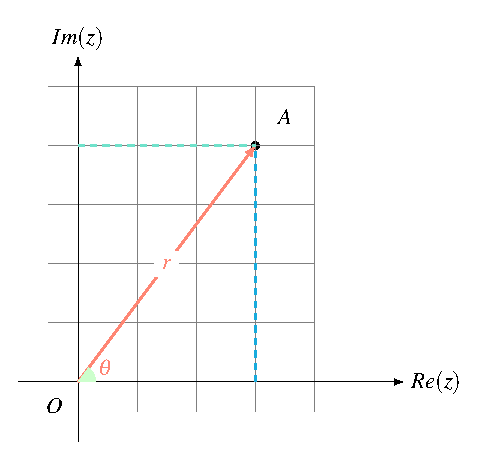
\includegraphics[width=0.8\textwidth]{agrand diagram}
\label{fig:argand 34}
\caption{复数z在复平面对应的点(位置矢量)}
\end{figure}

借此将复数赋予了几何含义——``复平面上的点,或者该点的位置矢量'';细细评估一下,和数轴上的点的概念非常类似。

因此也可以利用矢量形式写成$z=\vec{OA}=\icol{a\\b}$

\subsection*{复数的模与幅角}
复数的基本表示方案是$z=a+\mathbf{i} b$的形式,这种形式也被称之为Cartesian Form;当时当我们赋予了复数作为复平面上的位置矢量的时候,复数的\gls{modulus},计作$|z|$,其实也就是该对应矢量的模,因此可以用矢量相关概念做类似的推导。
\[
	|z|=|a+\mathbf{i} b|=\sqrt{a^2+b^2}
\]
一个复数的\gls{arg}就是该矢量与实轴的\emph{正}方向的夹角
\[
	\text{arg(z)}=\theta = \arctan \frac{b}{a}
\]
\begin{TaskBox}
求算\ref{fig:argand 34}当中,$A$对应复数的模和幅角
\end{TaskBox}

\subsection*{极坐标形式和欧拉公式}
而陈述一个复数的modulus和argument也能够帮助我们确定一个复数在复平面上的位置;可以计作$z=r\cdot (\cos \theta + \mathbf{i} \sin \theta)$。这种形式就是极坐标表示方案。

\subsubsection*{欧拉公式}
数学里的无冕之王,独眼巨人,勤奋的天才——欧拉,关于复数运算提出了非常著名欧拉公式:
\[
	e^{\mathbf{i} \theta} =\cos \theta +\mathbf{i} \sin\theta
\]
证明过程无需掌握,但是该公式是被誉为最美的数学公式之一。
\begin{figure}[H]
\centering
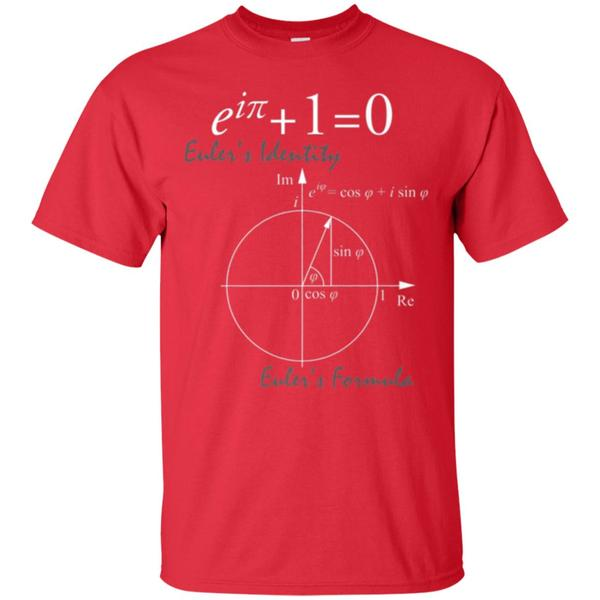
\includegraphics[width=0.8\textwidth]{EulerIden}
\end{figure}

因此在欧拉公式的加持下Polar Form可以改写为更简单的指数形式:
\[
	z=r\cdot (\cos \theta + \mathbf{i} \sin \theta)= r\cdot e^{\mathbf{i} \theta}
\]

\subsection*{复数加减的几何意义}
了解过几何含义之后,我们再重新看一下复数的加减法:如果有两个复数分别为$z_1=x_1 + \mathbf{i} y_1$ 和 $z_2=x_2 + \mathbf{i} y_2$,这两个复数之和$z_1+z_2=(x_1+x_2) +\mathbf{i}(y_1+y_2)$。将其改写为矢量形式$\icol{x_1\\y_1} + \icol{x_2\\y_2} =\icol{x_1+x_2 \\ y_1+y_2}$。再放入到复平面当中,如下图所示:
\begin{figure}[H]
\centering
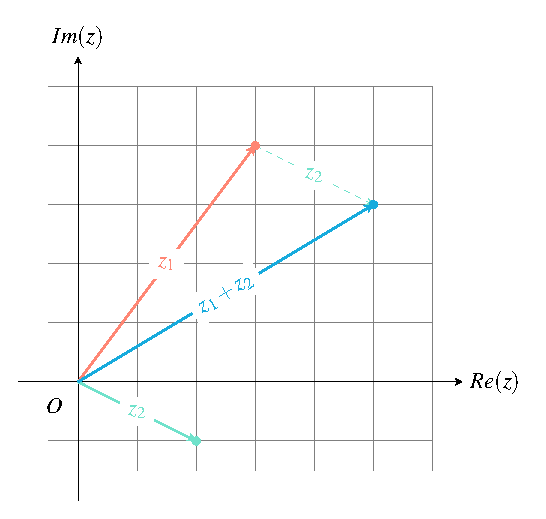
\includegraphics[width=0.8\textwidth]{addition complex}
\caption{两个复数之和在复平面上的体现}
\end{figure}

因此复数的加减法的几何意义就是\textbf{对应的矢量进行加减}。

\subsection*{乘除法的几何意义}
利用欧拉公式描述两个复数$z_1=r_1\cdot e^{\mathbf{i} \theta_1}$和$z_2=r_2\cdot e^{\mathbf{i} \theta_2}$。将这两个复数相乘是可以使用指数运算法则的。
\[
	z_1\cdot z_2 = r_1e^{\mathbf{i} \theta_1} \cdot  r_2e^{\mathbf{i} \theta_2} = r_1r_2 \cdot e^{\mathbf{i}( \theta_1+\theta_2)}
\]
也就是说,两个复数相乘的最终结果,其模等于各自的\textbf{模的乘积},其幅角等于各自\textbf{幅角之和};因而,如果两个复数相除,其结果的模等于各自的模之商,其幅角等于两个幅角之差。这就是复数的乘法的几何含义。

\subsection*{棣莫弗公式与欧拉公式与开根}
\label{subsec:De moivre}
当我们计算一个复数的$n$次方的时候,棣莫弗公式De Moivre Formula就会非常高效了:
\[
	z^n=r^n \cdot \left[\cos(n\theta) +\mathbf{i} \sin(n\theta) \right],\quad  \text{given that }z=r\left[\cos\theta +\mathbf{i} \sin\theta \right]
\]

该表达式的证明完全可以来自于欧拉公式,或者乘法的几何意义,亦或者来自于\emph{数学归纳法}

棣莫弗公式一个重大运用就是推导$\cos$ 和 $\sin$的$n$倍角公式;这个在STEP里面是一个基本功底;第二个运用就是用于求算复数的开根;因为只需要把$n$次方改写为分数次幂就可以了。现在开始证明\ref{subsec:polysolution}中$x^3=-8$这个方程的求解。
\begin{ExampleBox}
 首先,将右边的$-8$改写为复数的形式$z=-8+0\mathbf{i}$,再改写成极坐标形式$r=8,\theta=\pi$,再改写为指数的形式$z=8\cdot e^{\pi\mathbf{i}}$。
 因此根据$x$和右边复数$z$的立方关系。易得:
 \[
 	x=\sqrt[3]{z} \text{ or } x=z^{\frac{1}{3}}
 \]
 所以,利用De Moivre Formula, $|x|=\sqrt[3]{8}=2, \text{arg} x =\frac{\pi}{3}$。所以这样的话,就得到了其中的一个解 $x=2 e^{\frac{\pi}{3} \mathbf{i}}$。将其转变为常见的Cartesian Form就是$x= 2\cos(\frac{\pi}{3})+2\sin(\frac{\pi}{3})\mathbf{i}=1+\sqrt{3}\mathbf{i}$。

 等等,是不是好像有哪里不对的地方。我们明明还有$x=-2$和$x=1-\sqrt{3}\mathbf{i}$这两个解。这里只计算出一个。原因很简单,$\theta =\text{arg} z=\pi$这是符合我们最简化的写法的,但是考虑到幅角的\emph{周期性},实际上求算复数开根的时候,完全可以在原有的基础上加上$2\pi$。因此第二个解就是$x= 2\cos(\frac{\pi+2\pi}{3})+2\sin(\frac{\pi+2\pi}{3})\mathbf{i}=2$。那么我们再继续加上$2\pi$,就得到了第三个解$x= 2\cos(\frac{\pi+4\pi}{3})+2\sin(\frac{\pi+4\pi}{3})\mathbf{i}=1-\sqrt{3}\mathbf{i}$。

 至此,该方程的三个解全部解出。再继续加$2\pi$会重复之前的结果。其根出现在一个模为$2$,间隔为$\frac{2\pi}{3}$的单位圆上。
 \begin{figure}[H]
 \centering
 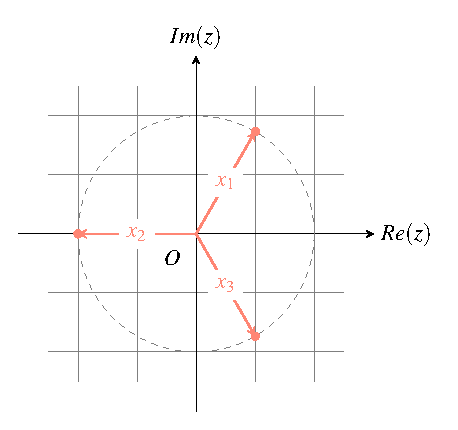
\includegraphics[width=0.8\textwidth]{cubicroot}
 \end{figure}
 是不是非常的amazing啊。
\end{ExampleBox}
\clearpage


\section{复数的Locus}
现在,我们的自变量就可以从实数领域的$x$变成复数领域的$z$。当我们建立一些方程或者不等式的时候,把满足要求的所有复数$z$在复平面上体现出来,就会得到这些复数的轨迹图。这些轨迹图像往往都是有特定的几何含义的。让我们一一进行探讨。

\subsection*{轨迹圆}
形如:
\[
	|z-(a+b\mathbf{i})|=r \qquad |z-(a+b\mathbf{i})|\leqslant r
\]
表达式或者不等式,会形成一个以$(a+b\mathbf{i})$所代表的点为圆心,以$r$为半径的圆。

\begin{figure}[H]
\centering
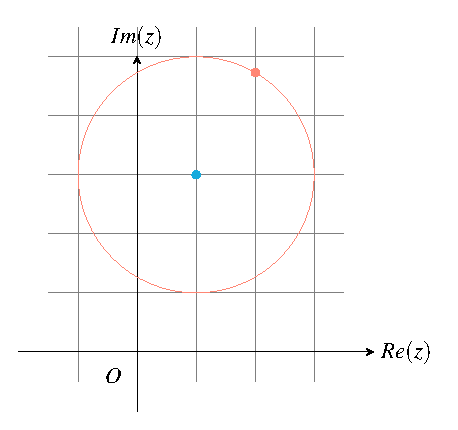
\includegraphics[width=0.4\textwidth]{complex circle}
\end{figure}

\begin{TaskBox}
完成上图的loci表达式,明确半径和圆心所代表的复数;
考虑一下等于符号,和不等符号的对结果图像的联系和区别;
\end{TaskBox}

\subsection*{半直线}
形如:
\[
	arg(z-(a+b\mathbf{i}))=\theta
\]
的表达式,代表复平面的上经过$(a+b\mathbf{i})$,并且与$x$轴方向的水平夹角为$\theta$。

\begin{figure}[H]
\centering
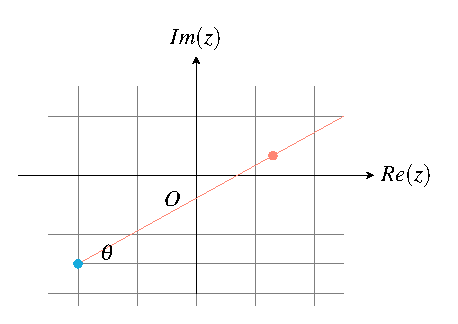
\includegraphics[width=0.8\textwidth]{complexline}
\end{figure}

\subsection*{中垂线}
形如:
\[
	|z-(a_1+b_1\mathbf{i})| = |z-(a_2+b_2\mathbf{i})|
\]
的表达式,则是代表复平面上,到两个点$(a_1+b_1\mathbf{i})$和$(a_2+b_2\mathbf{i})$的距离相等的复数,因此这些满足要求的复数其实就构成了线段的\textbf{垂直平分线}

\begin{figure}[H]
\centering
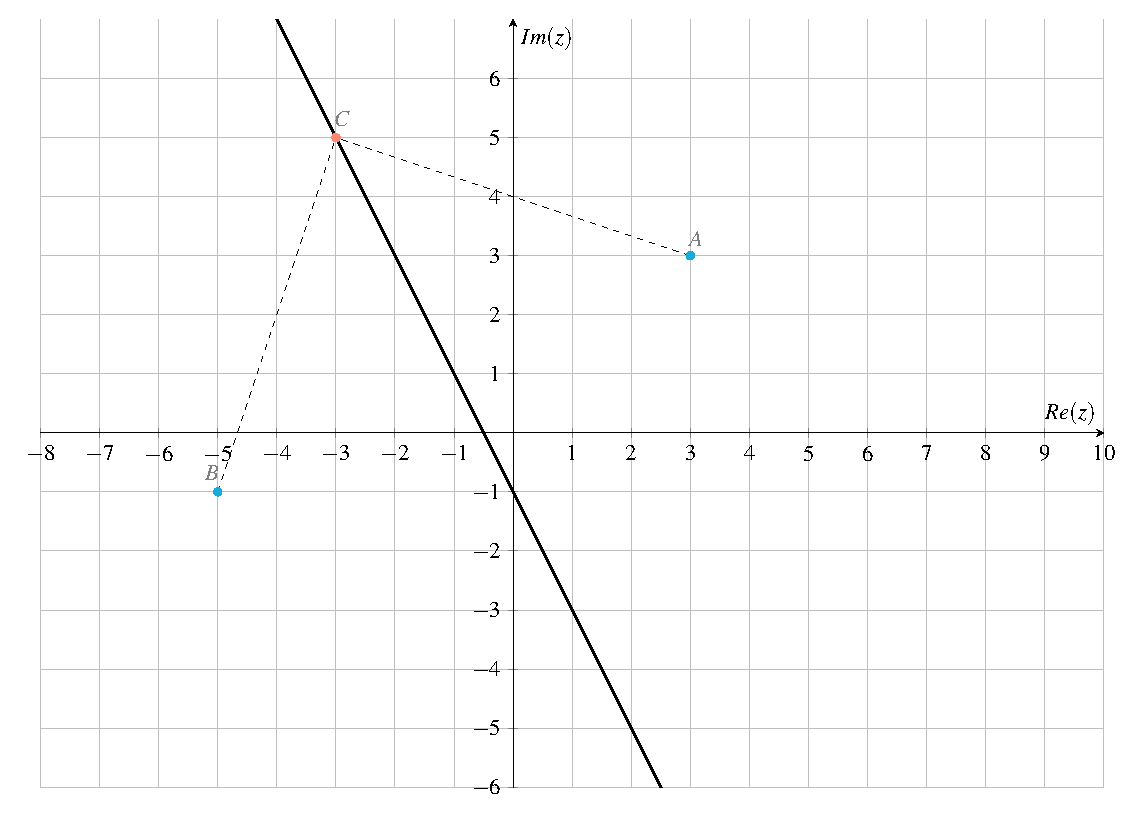
\includegraphics[width=0.8\textwidth]{perpendicular}
\end{figure}

